\documentclass[a4paper,11pt]{article}
\usepackage[utf8]{inputenc}
\usepackage{amsmath}
\usepackage{amsfonts}
\usepackage{amssymb}
\usepackage{graphicx}
\usepackage{braket}

\numberwithin{equation}{section}
\renewcommand\thesubsection{\alph{subsection}}
\newcommand{\bvp}[1]{\mathbf{#1}'}
\newcommand{\bv}[1]{\mathbf{#1}}
\newcommand{\ez}{\epsilon_0}
\newcommand{\eo}{\epsilon_1}
\newcommand{\lrp}[1]{\left({#1}\right)}
\newcommand{\lrb}[1]{\left\{{#1}\right\}}


%opening
\title{Solid State 1 HW4}
\author{Geoffrey Xiao, Vincent Baker, Eli Worth}

\begin{document}
\maketitle

\section*{Q1}
1) We consider the vertical displacements of the atoms from equilibrium.
We assume that the potential energy function near equilibirum is approximately quadratic, and therefore the force is approximately linear.
with constant of porportionality C. 
The complete expression for the force on the center atom has contributions from each of the nearest neighbors:
\begin{align}
 \begin{split}
 F = C\{&(u_{n-1,m}-u_{n,m})+(u_{n+1,m}-u_{n,m})\\
      &+(u_{n,m-1}-u_{n,m})+(u_{n,m+1}-u_{n,m})\}
 \end{split}\\
 F &= C\lrp{u_{n-1,m}+u_{n+1,m}+u_{n,m-1}+u_{n,m+1}-4u_{n,m}}
\end{align}
2) The equation of motion is:
\begin{align}
 M\frac{d^2u_{n,m}}{dt^2} &= C\lrp{u_{n-1,m}+u_{n+1,m}+u_{n,m-1}+u_{n,m+1}-4u_{n,m}}
\end{align}
3) We assume a solution of the form:
\begin{align}
 u_{n,m} &= u_0e^{ink_xa}e^{imk_ya}e^{-i\omega t}\\
 u_{n\pm1,m} &= u_0e^{ink_xa}e^{imk_ya}e^{-i\omega t}e^{\pm ik_xa}\\
 u_{n,m\pm 1} &= u_0e^{ink_xa}e^{imk_ya}e^{-i\omega t}e^{\pm ik_ya}\\
\end{align}
We note that the $n\pm 1, m\pm 1$ expressions are just $u_{n,m}$ multiplied by $e^{\pm ik_xa},e^{\pm ik_ya}$.
The second time derivate brings down a factor $-\omega^2$, so (0.3) becomes:
\begin{align}
 -M\omega^2u_{n,m} &= Cu_{n,m}\lrp{e^{ik_xa}+e^{-ik_xa}+e^{ik_ya}+e^{-ik_ya}-4}\\
 \omega^2 &= 2C/M\lrp{2-\cos{k_xa}-\cos{k_ya}}\\
 \omega &= \sqrt{4C/M}\lrp{1-\cos{\frac{(k_x+k_y)a}{2}}\cos{\frac{(k_x-k_y)a}{2}} }^{1/2}
\end{align}
\\
The dispersion relation is shown in figure 1.
\begin{figure}[h]
 \caption{Dispersion relation}
 \centering
   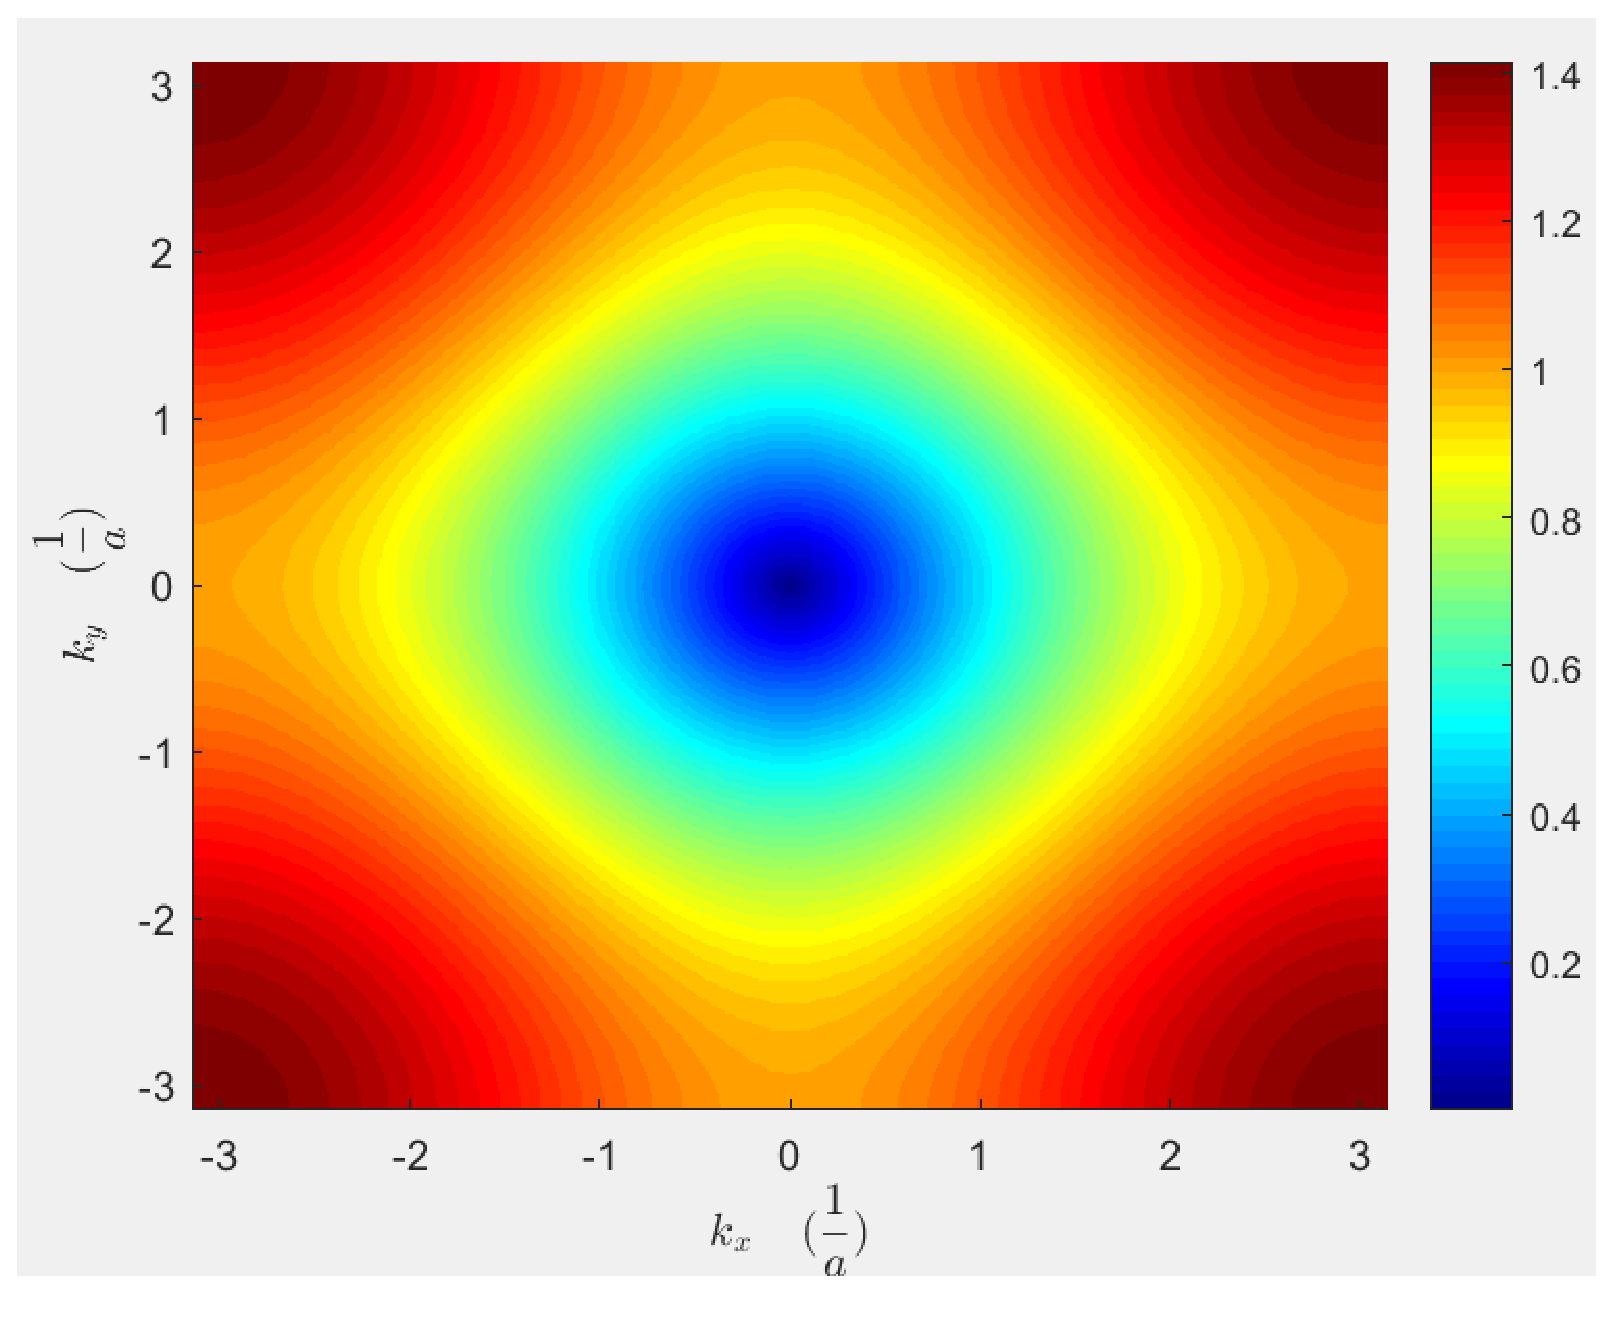
\includegraphics[width=\textwidth]{p1}
\end{figure}
\\
\section*{Q2}
Measuring phonon dispersion requires exciting phonon modes through inelastic collisions.
Neutrons are neutral and therefore interact mostly with the atomic nucleii rather than the electron clouds.
This nuclear position displacement is what can excite phonon modes.
Because neutrons are massive compared to electrons, the energy $E=\hbar^2k^2/2M$ is lower than an electron of the same momentum.
In the conservation of energy equation:
\begin{align}
 \frac{\hbar^2k^2}{2M_N} &= \frac{\hbar^2k'^2}{2M_N}\pm\hbar\omega
\end{align}
This implies that a neutron can excite lower energy phonons for the same $\Delta k$ as an electron.
Since phonons (especially acoustic phonons) are relatively low energy, neutrons may more readily probe the phonon modes.






\end{document}
